\documentclass{article}

\usepackage{amsmath}
\usepackage{amssymb}
\usepackage{amsthm}
\usepackage{bpextra}
\usepackage{float}
\usepackage{geometry}
\usepackage{latexsym}
\usepackage{natbib}
\usepackage{pdfpages}
\usepackage{subcaption}
\usepackage{tikz}
\usepackage{tkz-berge}
\usepackage{varwidth}

% tikz things
\usetikzlibrary{petri, topaths, positioning, decorations.pathmorphing}

% natbib source
\bibliographystyle{agsm}
\renewcommand{\bibsection}{}

\pgfarrowsdeclare{arr}{arr}{
    \setlength{\arrowsize}{2\pgflinewidth}
    \addtolength{\arrowsize}{.5\pgflinewidth}
    \pgfarrowsrightextend{-1\arrowsize}
    \pgfarrowsleftextend{1\arrowsize}
}{
    \setlength{\arrowsize}{2\pgflinewidth}
    \addtolength{\arrowsize}{.5\pgflinewidth}
    \pgfpathmoveto{\pgfpoint{-5\arrowsize}{4\arrowsize}}
    \pgfpathlineto{\pgfpointorigin}
    \pgfpathlineto{\pgfpoint{-5\arrowsize}{-4\arrowsize}}
    \pgfusepathqstroke
}

\newcommand{\drawsquig}{\draw[-arr,
line join=round,
decorate, decoration={
    zigzag,
    segment length=4,
    amplitude=.9,post=lineto,
    post length=2pt
}]}

\newenvironment{scprooftree}[1]%
  {\gdef\scalefactor{#1}\begin{center}\proofSkipAmount \leavevmode}%
  {\scalebox{\scalefactor}{\DisplayProof}\proofSkipAmount \end{center} }


\newcommand\vc[1]{\vcenter{\hbox{#1}}}

\newcommand\atom[1]{%
 \ifx#11a\else%
 \ifx#12b\else%
 \ifx#13c\else%
 \fi\fi\fi
}

\newcommand\0{0}
\newcommand\1{1}
\newcommand\+{+}
\renewcommand\*{\times}

\newcommand{\tightplus}{\!+\!}
\newcommand{\tighttimes}{\!\*\!}
\newcommand\subs[1]{\mathsf{|#1|}}

\tikzstyle{tok}=[circle,inner sep=0pt,minimum size=4pt,outer sep=1pt]
\tikzstyle{src}=[black,text height=1ex,text depth=0ex,rotate=90]
\tikzstyle{tgt}=[black,text height=1ex,text depth=0ex]%,rotate=-45]
\tikzstyle{for}=[text height=1.5ex,text depth=.25ex]
\tikzstyle{jmp}=[->,line width=1pt,cap=round,gray]
\tikzstyle{jmp1}=[jmp]
\tikzstyle{jmp2}=[jmp,red]

\tikzstyle{tokB}=[fill,tok]
\tikzstyle{tokG}=[fill,tok,gray]
\tikzstyle{tokR}=[fill,tok,red]
\tikzstyle{tokRed}=[fill,tok,red]
\tikzstyle{tokBlue}=[fill,tok,blue]
\tikzstyle{tokGreen}=[fill,tok,darkgreen]
\tikzstyle{tokF}=[draw,thick,gray,circle,inner sep=0pt, minimum size=7pt]

\tikzstyle{matrix}=[x=-5mm,y=5mm,rotate=-90]

% delta-equals (unused)
\def\deltaeq{\mathrel{\ensurestackMath{\stackon[1pt]{=}{\scriptstyle\Delta}}}}
% define-equals
\def\defeq{::=}
% set-to-equals
\def\seteq{:=}

\newcommand\dual{\overline}

\title{From Additive to Classical Proof Search}
\date{}



\author{Adam Lassiter\\Department of Computer Science\\University of Bath \and Willem Heijltjes\\Department of Computer Science\\University of Bath}
\usepackage{enumitem}
\usepackage[hidelinks]{hyperref}
\usepackage{titlesec}

\titlespacing{\section}{0pt}{12pt plus 4pt minus 2pt}{0pt plus 2pt minus 2pt}


\begin{document}
    {\let\newpage\relax\maketitle}

    \maketitle


    \section*{Introduction}
        Building on the work done by \citet{petri-nets}, we investigate proof search in Classical Logic (CL) through Additive Linear Logic (ALL).
        The process we investigate, called \emph{coalescence}, is a top-down proof search from axiom links down to the conclusion.
        This method is promising as it boasts great efficiency for ALL proof search and has a natural transformation to sequent calculus proofs.
        The interesting features are that: proof search steps are simple, $\mathcal{O}(n)$, there is no need for backtracking, the method has built-in sharing (or memoization); but dimensionality increases rapidly, and sometimes unexpectedly.



    \section*{Additive Linear Logic}
        ALL is the fragment of linear logic that concerns sum $(+)$ and product $(\*)$, with their units $0$ and $1$.
        A \emph{formula} of ALL is constructed:
        \begin{equation*}
            A, B, C \quad \defeq \quad 0 \mid 1 \mid a \mid \dual a \mid A + B \mid A \* B
        \end{equation*}
        We write $\subs A$ for the set of subformula occurrences of $A$ (we distinguish uniquely both occurrences of $a$ in $a\*a$).

        A sequent for ALL is a pair $\vdash A,B$, and a sequent calculus for ALL is given by the following rules (where the symmetric rules operating on the second element of the pair $\vdash A,B$ are omitted):
        \begin{figure}[H]
            \centering
            \begin{minipage}{0.3\linewidth}
                \begin{prooftree}
                    \AxiomC{~}
                    \RightLabel{$ax$}
                    \UnaryInfC{$\vdash a,\dual a$}
                \end{prooftree}
            \end{minipage}
            \begin{minipage}{0.3\linewidth}
                \begin{prooftree}
                    \AxiomC{~}
                    \RightLabel{$\1$}
                    \UnaryInfC{$\vdash \1,A$}
                \end{prooftree}
            \end{minipage}
            \begin{minipage}{0.3\linewidth}
                \begin{prooftree}
                    \AxiomC{$\vdash A,C$}
                    \RightLabel{$\+_1$}
                    \UnaryInfC{$\vdash A\+B,C$}
                \end{prooftree}
            \end{minipage}

            \begin{minipage}{0.4\linewidth}
                \begin{prooftree}
                    \AxiomC{$\vdash B,C$}
                    \RightLabel{$\+_2$}
                    \UnaryInfC{$\vdash A\+B,C$}
                \end{prooftree}
            \end{minipage}
            \begin{minipage}{0.4\linewidth}
                \begin{prooftree}
                    \AxiomC{$\vdash A,C$}
                    \AxiomC{$\vdash B,C$}
                    \RightLabel{$\*$}
                    \BinaryInfC{$\vdash A\*B,C$}
                \end{prooftree}
            \end{minipage}
        \end{figure}



    \section*{Coalescence Proof Search}
        Naively searching for a sequent proof, starting from a given conclusion, is exponential: the additive conjunction rule $(\*)$ duplicates its context $C$, and reciprocated duplication between both formulas in the sequent creates exponential growth.
        A more efficient algorithm, first observed by \citet{semantic-methods} and later by \citet{petri-nets}, is given by placing proof search for a sequent $\vdash A,B$ in the product space $\subs A\* \subs B$.
        This set contains all \emph{sub-sequents} of $\vdash A,B$ that might occur in a sequent proof of $\vdash A,B$, without redundancy.
        We represent $\subs A\* \subs B$ by a grid, e.g.\ that for $\vdash \dual a\+(\dual b\+\dual c),(a\* b)\*c$ is below:
        \[
            \vc{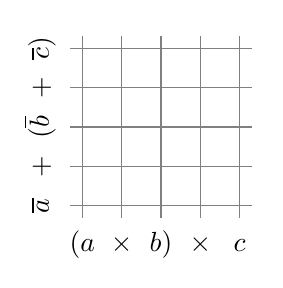
\begin{tikzpicture}[matrix]
                \foreach \x/\a in {1/\dual{\atom1}, 2/\+, 3/(\dual{\atom2}, 4/\+, 5/\dual{\atom3})}%
                    \draw[gray] (\x,0) node[src] {$\a$} (\x,.7) -- (\x,5.3);
                \foreach \y/\b in {1/(\atom1, 2/\*, 3/\atom2), 4/\*, 5/\atom3}%
                    \draw[gray] (0,\y) node[tgt] {$\b$} (.7,\y) -- (5.3,\y);
            \end{tikzpicture}}
            \quad\rightsquigarrow\quad
            \vc{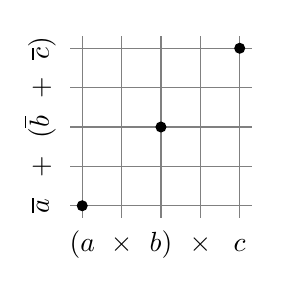
\begin{tikzpicture}[matrix]
                \foreach \x/\a in {1/\dual{\atom1}, 2/\+, 3/(\dual{\atom2}, 4/\+, 5/\dual{\atom3})}%
                    \draw[gray] (\x,0) node[src] {$\a$} (\x,.7) -- (\x,5.3);
                \foreach \y/\b in {1/(\atom1, 2/\*, 3/\atom2), 4/\*, 5/\atom3}%
                    \draw[gray] (0,\y) node[tgt] {$\b$} (.7,\y) -- (5.3,\y);
                \foreach \p/\n in { {1,1}/a1, {3,3}/b1, {5,5}/c1} \node[tokB] (\n) at (\p) {};
            \end{tikzpicture}}
        \]

        The \emph{coalescence proof search} algorithm for ALL is then as follows.
        We place tokens on this grid to indicate a sub-sequent is provable.
        We initially place tokens on each position $(\dual a,a)$, $(\1,A)$, and $(A,\1)$, as shown above right for our example, then apply the following local rules (and the symmetric variants):
        \begin{itemize}[noitemsep]
            \item Place a token on $(A\+B,C)$ if $(A,C)$ has a token.
            \item Place a token on $(A\+B,C)$ if $(B,C)$ has a token.
            \item Place a token on $(A\*B,C)$ if $(A,C)$ and $(B,C)$ have a token.
        \end{itemize}

        We illustrate these graphically as follows; note, though, that the \emph{neighbours} of a position in the grid are given by the subformula relation, and not by adjacency in the plane:
        \[
            \def\dual{}
            \begin{array}{cccccc}
                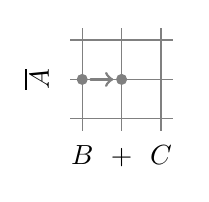
\begin{tikzpicture}[matrix]
                    \foreach \i/\a in {1/{}, 2/\dual A, 3/{}}
                        {\draw[gray] (\i,0) node[src] {$\a$} (\i,.7) -- (\i,3.3);}
                    \foreach \j/\b in {1/B, 2/\+, 3/C}
                        {\draw[gray] (0,\j) node[tgt] {$\b$} (.7,\j) -- (3.3,\j);}
                    \node[tokG] (a) at (2,1) {};
                    \node[tokG] (c) at (2,2) {};
                    \draw[jmp1] (a) to (c);
                \end{tikzpicture}
                &
                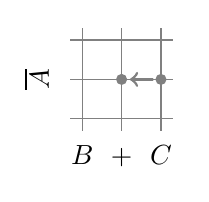
\begin{tikzpicture}[matrix]
                    \foreach \i/\a in {1/{}, 2/\dual A, 3/{}}
                        {\draw[gray] (\i,0) node[src] {$\a$} (\i,.7) -- (\i,3.3);}
                    \foreach \j/\b in {1/B, 2/\+, 3/C}
                        {\draw[gray] (0,\j) node[tgt] {$\b$} (.7,\j) -- (3.3,\j);}
                    \node[tokG] (b) at (2,3) {};
                    \node[tokG] (c) at (2,2) {};
                    \draw[jmp1] (b) to (c);
                \end{tikzpicture}
                &
                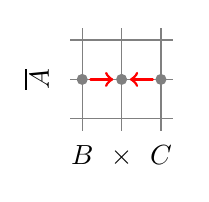
\begin{tikzpicture}[matrix]
                  \foreach \i/\a in {1/{}, 2/\dual A, 3/{}}
                    {\draw[gray] (\i,0) node[src] {$\a$} (\i,.7) -- (\i,3.3);}
                  \foreach \j/\b in {1/B, 2/\*, 3/C}
                    {\draw[gray] (0,\j) node[tgt] {$\b$} (.7,\j) -- (3.3,\j);}
                  \node[tokG] (a) at (2,1) {};
                  \node[tokG] (b) at (2,3) {};
                  \node[tokG] (c) at (2,2) {};
                  \draw[jmp2] (a) to (c);
                  \draw[jmp2] (b) to (c);
                \end{tikzpicture}
                &
                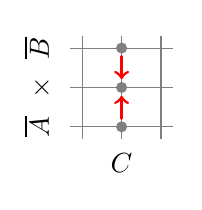
\begin{tikzpicture}[matrix]
                    \foreach \i/\a in {1/\dual A, 2/\*, 3/\dual B}
                        {\draw[gray] (\i,0) node[src] {$\a$} (\i,.7) -- (\i,3.3);}
                    \foreach \j/\b in {1/{}, 2/C, 3/{}}
                        {\draw[gray] (0,\j) node[tgt] {$\b$} (.7,\j) -- (3.3,\j);}
                    \node[tokG] (a) at (1,2) {};
                    \node[tokG] (b) at (3,2) {};
                    \node[tokG] (c) at (2,2) {};
                    \draw[jmp2] (a) to (c);
                    \draw[jmp2] (b) to (c);
                \end{tikzpicture}
                &
                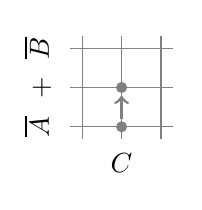
\begin{tikzpicture}[matrix]
                    \foreach \i/\a in {1/\dual A, 2/\+, 3/\dual B}
                        {\draw[gray] (\i,0) node[src] {$\a$} (\i,.7) -- (\i,3.3);}
                    \foreach \j/\b in {1/{}, 2/C, 3/{}}
                        {\draw[gray] (0,\j) node[tgt] {$\b$} (.7,\j) -- (3.3,\j);}
                    \node[tokG] (a) at (1,2) {};
                    \node[tokG] (c) at (2,2) {};
                    \draw[jmp1] (a) to (c);
                \end{tikzpicture}
                &
                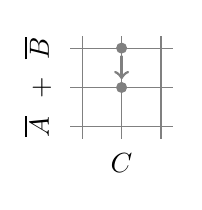
\begin{tikzpicture}[matrix]
                    \foreach \i/\a in {1/\dual A, 2/\+, 3/\dual B}
                        {\draw[gray] (\i,0) node[src] {$\a$} (\i,.7) -- (\i,3.3);}
                    \foreach \j/\b in {1/{}, 2/C, 3/{}}
                        {\draw[gray] (0,\j) node[tgt] {$\b$} (.7,\j) -- (3.3,\j);}
                    \node[tokG] (b) at (3,2) {};
                    \node[tokG] (c) at (2,2) {};
                    \draw[jmp1] (b) to (c);
                \end{tikzpicture}
            \end{array}
        \]
        Observe also that the initial token placement and the propagation rules correspond directly to the axioms and sequent rules for ALL respectively.

        Finally, if the root position $(A,B)$ for $\vdash A,B$ has a token, we succeed; otherwise, if no more tokens can be placed we fail.
        For our example, we get the following trace:
        \[
            \vc{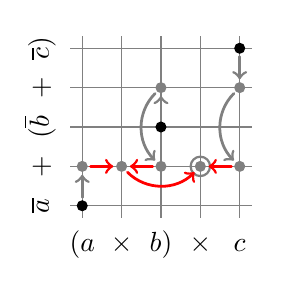
\begin{tikzpicture}[matrix]
                \foreach \x/\a in {1/\dual{\atom1}, 2/\+, 3/(\dual{\atom2}, 4/\+, 5/\dual{\atom3})}%
                    \draw[gray] (\x,0) node[src] {$\a$} (\x,.7) -- (\x,5.3);
                \foreach \y/\b in {1/(\atom1, 2/\*, 3/\atom2), 4/\*, 5/\atom3}%
                    \draw[gray] (0,\y) node[tgt] {$\b$} (.7,\y) -- (5.3,\y);
                \foreach \p/\n in {
                    {2,1}/a2, {2,2}/ab,
                    {4,3}/b2, {2,3}/b3,
                    {4,5}/c2, {2,5}/c3%
                } \node[tokG] (\n) at (\p) {};
                \node[tokG] (abc) at (2,4) {};
                \node[circle,draw,gray,thick,inner sep=0pt,minimum size=7pt] at (2,4) {};
                \foreach \p/\n in { {1,1}/a1, {3,3}/b1, {5,5}/c1} \node[tokB] (\n) at (\p) {};
                \foreach \s/\t in { a1/a2, b1/b2, c1/c2} \draw[jmp1] (\s)--(\t);
                \foreach \s/\t in { a2/ab, b3/ab, c3/abc} \draw[jmp2] (\s)--(\t);
                \draw[jmp1,bend right=45] (b2) to (b3);
                \draw[jmp1,bend right=45] (c2) to (c3);
                \draw[jmp2,bend right=45] (ab) to (abc);
            \end{tikzpicture}}
        \]

        This algorithm succeeds if and only if there is an ALL proof of the given formula.
        Clearly, each progression is local (i.e.\ constant time), and the number of tokens placed is bounded by the size of the grid $\subs A\times\subs B$.
        The algorithm thus runs in polynomial time.
        The interesting observation is that, naively, the additive, context-duplicating conjunction rule seems very inefficient for proof search.
        The coalescence approach solves this problem by using a natural data structure, the grid, to obtain an algorithm with natural memoization, that is efficient for this reason.



    \section*{Classical Logic and Coalescence}
        We investigate how the coalescence technique applies to classical propositional logic.
        The main idea is that a classical formula $A$ can be proved by additive rules applied to a sequent $\vdash A,\dots,A$ with $n$ copies of $A$.
        This is easily shown by a \emph{stratification} of sequent proofs with additive rules, where all contractions are pushed to the bottom (conclusion), and weakenings to the top (axioms).

        Correspondingly, we generalize coalescence proof search to CL by applying it to a grid of $n$ dimensions, for any $n$, where it was previously fixed at $2$.
        The algorithm will start at dimension $1$, and when it fails at dimension $n$ it will try again at dimension $n+1$, up to a theoretically determined upper bound.
        A \emph{formula} within CL is constructed:
        \begin{equation*}
            A, B, C \quad \defeq \quad \top \mid \bot \mid a \mid \dual a \mid A \vee B \mid A \wedge B
        \end{equation*}

        A sequent calculus for CL is then given by the following rules:
        \begin{figure}[H]
            \centering
            \begin{minipage}[H]{.3\linewidth}
                \begin{prooftree}
                    \AxiomC{~}
                    \RightLabel{$\top$}
                    \UnaryInfC{$\vdash \top$}
                \end{prooftree}
            \end{minipage}
            \begin{minipage}[H]{.3\linewidth}
                \begin{prooftree}
                    \AxiomC{$\vdash \Gamma, A$}
                    \RightLabel{$\vee$}
                    \UnaryInfC{$\vdash \Gamma, A \vee B$}
                \end{prooftree}
            \end{minipage}
            \begin{minipage}[H]{.3\linewidth}
                \begin{prooftree}
                    \AxiomC{$\vdash \Gamma$}
                    \RightLabel{$w$}
                    \UnaryInfC{$\vdash \Gamma, A$}
                \end{prooftree}
            \end{minipage}

            \begin{minipage}[H]{.3\linewidth}
                \begin{prooftree}
                    \AxiomC{~}
                    \RightLabel{$ax$}
                    \UnaryInfC{$\vdash a, \dual a$}
                \end{prooftree}
            \end{minipage}
            \begin{minipage}[H]{.3\linewidth}
                \begin{prooftree}
                    \AxiomC{$\vdash \Gamma, A$}
                    \AxiomC{$\vdash \Gamma, B$}
                    \RightLabel{$\wedge$}
                    \BinaryInfC{$\vdash \Gamma, A \wedge B$}
                \end{prooftree}
            \end{minipage}
            \begin{minipage}[H]{.3\linewidth}
                \begin{prooftree}
                    \AxiomC{$\vdash \Gamma, A, A$}
                    \RightLabel{$c$}
                    \UnaryInfC{$\vdash \Gamma, A$}
                \end{prooftree}
            \end{minipage}
        \end{figure}
        \noindent where $A, B, C$ are formulae and $\Gamma, \Delta, \Sigma$ are sequents.
        Notice that both conjunction $\wedge$ and disjunction $\vee$ rules preserve the number of terms in a sequent, but there is no longer a bound on the number of terms per sequent through the weakening $w$ and contraction $c$ rules.

        A proof tree is said to be \emph{additively stratified} if it is structured as follows:
        \begin{prooftree}
            \AxiomC{}
            \RightLabel{$\top, ax$}\doubleLine\UnaryInfC{$\vdash A_1$}
            \RightLabel{$w$}\doubleLine\UnaryInfC{$\vdash \Gamma_1$}
            \AxiomC{\dots}
            \AxiomC{}
            \RightLabel{$\top, ax$}\doubleLine\UnaryInfC{$\vdash A_n$}
            \RightLabel{$w$}\doubleLine\UnaryInfC{$\vdash \Gamma_n$}
            \RightLabel{$\wedge, \vee$}\doubleLine\TrinaryInfC{$\vdash P \dots P$}
            \RightLabel{$c$}\doubleLine\UnaryInfC{$\vdash P$}
        \end{prooftree}
        That is, any proof tree in CL sequent calculus may be rearranged such that rules applied are ordered $\{\top, ax\}, w, \{\vee, \wedge\}, c$.
        This rearrangement does not affect the number of terms of sequents.

        For a formula $P$ in CL, the coalescence algorithm runs as follows:
        \begin{enumerate}[noitemsep]
            \item Set $n := 1$
            \item\label{l} Construct the $n$-dimensional grid of possible $n$-term sequents $\vdash A_1 \dots A_n \in \subs A \* \dots_n \* \subs A$
            \item Spawn tokens at all instances of axiom links $\vdash \Gamma, a, \dual a$
            \item Exhaustively perform transitions given by the CL sequent calculus rules
            \item Does there exist a token at $(P, P \dots P) \equiv \,\, \vdash P, P \dots P \equiv \,\, \vdash P$?
            \begin{enumerate}[noitemsep]
                \item Yes --- Halt with a proof for $P$ and dimensionality $n$
                \item No --- Increment $n := n + 1$ and goto~\ref{l}
            \end{enumerate}
        \end{enumerate}
        The dimensionality of a proof is then the dimensionality of our grid when the root is reached, equivalent to the number of contractions required in an equivalent sequent proof.
        A CL formula can thus be proved by an $n$-dimensional additively stratified proof, where $n$ is the number of terms in a sequent before contraction.
        Through a natural transformation on steps of the algorithm to equivalent sequent proofs, coalescence up to $n = N$ is then exactly (additively stratified) proof search, with implicit weakening and contraction of all sequents up to $N$ terms.



    \section*{Some Examples}
        Consider a simple proof requiring disjunction through $A \defeq a \vee \dual a$ as follows:

        \newcommand\spawnIGrid[1]{\vc{\begin{tikzpicture}[matrix,x=-3.5mm,y=3.5mm]
                \foreach \x/\a in {1/\atom1, 2/\vee, 3/\dual{\atom1}} \draw[gray] (\x,0) node[src] {\footnotesize$\a$} (\x,.7) -- (\x,3.3);
                \foreach \y/\b in {1/\atom1, 2/\vee, 3/\dual{\atom1}} \draw[gray] (0,\y) node[tgt] {\footnotesize$\b$} (.7,\y) -- (3.3,\y);
                \foreach \p/\n/\c in {#1} \node[fill,tok,\c] (\n) at (\p) {};
            \end{tikzpicture}}}
        \newcommand\initSpawnIGrid{\spawnIGrid{{1,3}/a1/blue, {3,1}/b1/red}}

        \[
             \initSpawnIGrid
             \quad\rightsquigarrow\quad
             \spawnIGrid{{1,3}/a1/blue, {3,1}/b1/red, {2,3}/c1/blue}
             \quad\rightsquigarrow\quad
             \spawnIGrid{{1,3}/a1/blue, {3,1}/b1/red, {2,3}/c1/blue, {3,2}/d1/red}
             \quad\rightsquigarrow\quad
             \spawnIGrid{{1,3}/a1/blue, {3,1}/b1/red, {2,3}/c1/blue, {3,2}/d1/red, {2,2}/e1/blue}
        \]

        The root position $(A, A)$ is reached in 2 dimensions so we describe the associated proof as having dimensionality 2.
        Consider next a simple proof requiring conjunction through $B \defeq (a \vee \dual a) \wedge (b \vee \dual b)$ as follows (note intermediate steps are skipped and the grid is saturated before a proof is reached):

        \newcommand\spawnIIGrid[1]{\vc{\begin{tikzpicture}[matrix,x=-3.5mm,y=3.5mm]
                    \foreach \x/\a in {1/\atom1, 2/\vee, 3/\dual{\atom1}, 4/\wedge, 5/\atom2, 6/\vee, 7/\dual{\atom2}} \draw[gray] (\x,0) node[src] {\footnotesize$\a$} (\x,.7) -- (\x,7.3);
                    \foreach \y/\b in {1/\atom1, 2/\vee, 3/\dual{\atom1}, 4/\wedge, 5/\atom2, 6/\vee, 7/\dual{\atom2}} \draw[gray] (0,\y) node[tgt] {\footnotesize$\b$} (.7,\y) -- (7.3,\y);
                \foreach \p/\n/\c in {#1} \node[fill,tok,\c] (\n) at (\p) {};
            \end{tikzpicture}}}
        \newcommand\initSpawnIIGrid{\spawnIIGrid{{1,3}/a1/blue, {3,1}/b1/red, {5,7}/c1/black!10!cyan, {7,5}/d1/black!10!magenta}}

        \[
            \initSpawnIIGrid
            \quad\rightsquigarrow^*\quad
            \spawnIIGrid{{1,3}/a1/blue, {2,3}/a2/blue, {1,2}/a3/blue, {2,2}/a4/blue, {3,1}/b1/red, {3,2}/b2/red, {2,1}/b3/red, {5,7}/c1/black!10!cyan, {6,7}/c2/black!10!cyan, {5,6}/c3/black!10!cyan, {6,6}/c4/black!10!cyan, {7,5}/d1/black!10!magenta, {7,6}/d2/black!10!magenta, {6,5}/d3/black!10!magenta}
        \]

        We do not reach the root $(B, B)$ for $n = 2$ despite having two proven `subproofs' and need only apply a simple conjunction.
        Instead, a solution is reached for $n = 3$ (visualisation omitted due to lack of clarity of 3D diagrams).
        For a similar term in 3 variables $\atom1, \atom2, \atom3$, a solution is reached for $n = 4$ and growth continues linearly.
        This is deemend unsatisfying and we readdress the mechanics of coalescence to fix this.



    \section*{Current Work}
        To solve this issue, we then investigate liberating the search algorithm and generalising over the properties of sequents --- namely, idempotency and commutativity.
        This includes: some notion of applying conjunctions `diagonally' (from $(a \vee \dual a, b \vee \dual b)$ to ($B, B$) in one step in the above) and switching from \emph{tuple} or \emph{multiset} links to \emph{set} links.
        The latter takes us into more familiar/obvious proof search territory:
        \begin{figure}[H]
            \def\x{1cm}
            \def\y{1cm}
            \centering
            \begin{tikzpicture}
                \node[anchor=center](root){};
                \node[on grid, left=       2*\x of root   ](13){$\{a, \dual a\}$};
                \node[on grid, right=      2*\x of root   ](57){$\{b, \dual b\}$};
                \node[on grid, below left= \y and \x of 13](23){$\{a \vee \dual a, \dual a\}$};
                \node[on grid, below right=\y and \x of 13](12){$\{a, a \vee \dual a\}$};
                \node[on grid, below left= \y and \x of 57](67){$\{b \vee \dual b, \dual b\}$};
                \node[on grid, below right=\y and \x of 57](56){$\{b, b \vee \dual b\}$};
                \node[on grid, below right=\y and \x of 23](2){$\{a \vee \dual a\}$};
                \node[on grid, below right=\y and \x of 67](6){$\{b \vee \dual b\}$};
                \coordinate[on grid, below right=0.5\y and 2*\x of 2](4c){};
                \node[on grid, below=0.5\y of 4c](4){$\{(a \vee \dual a) \wedge (b \vee \dual b)\}$};

                \draw[-arr] (13) to (23);
                \draw[-arr] (13) to (12);
                \draw[-arr] (57) to (67);
                \draw[-arr] (57) to (56);
                \draw[-arr] (23) to (2);
                \draw[-arr] (12) to (2);
                \draw[-arr] (67) to (6);
                \draw[-arr] (56) to (6);
                \draw[-] (2) to (4c) to (6);
                \draw[-arr] (4c) to (4);
            \end{tikzpicture}
        \end{figure}

        Furthermore, we examine bounds on the dimension required for a given formula.
        We initially propose a trivial theoretical upper bound through number of unique atoms in a formula $A$.
        Through construction of a set of classes representing formulae provable in $n$ dimensions and a simple algebra of these classes, we hypothesise complexity is bounded by the largest disjunctive form in $\subs A$.



    \section*{References}
        \bibliography{dortmund}


\end{document}
